

% \subsection{問題設定}
% 本研究では,銀行のローンの審査システムについての機械学習モデルを想定し,認可拒否について誤分類を引き起こす敵対的サンプルを生成することを考える.銀行のローンを申請する顧客情報と正解データをもとに機械学習モデルが学習し,テストデータに対する分類結果を出力する.敵対的サンプルによる誤分類は,銀行にとってリスクの高いローンを誤って認可してしまう可能性がある.このような問題に対処するため,機械学習モデルの安全性が求められており,敵対的サンプルに対する防御手法が必要である.また同時に,モデルの脆弱性を理解することは,安全性を向上させるために重要である.

\subsection{敵対的学習}
敵対的学習は,機械学習モデルの堅牢性を向上させるための手法として誕生した。従来の機械学習モデルは、訓練データに対して高い精度を示す一方で、敵対的サンプルと呼ばれる微細ななノイズを含むデータに対しては脆弱である
ことが知られている。これにより、モデルが誤分類を引き起こし、セキュリティ上のリスクが生じる可能性がある。

goodfellowらの研究\cite{goodfellow2015explaining}でこの敵対的学習について提案された。この手法では、正常データと敵対的サンプルの特徴をAIに学習させる防御手法である。機械学習モデルの学習時において、正常データと敵対的サンプルに対する誤差(Loss)をそれぞれ計算し、これらを足し合わせた値を基のモデルの重み $\bm{w}$ を更新することで、敵対的サンプルの特徴を学習する。

以下に実際の敵対的学習の流れを示す。
\begin{enumerate}
    \item 学習中の機械学習モデルを利用して敵対的サンプルを作成する

    \item 機械モデルに正常なデータ $\bm{x}$ と敵対的サンプル $\bm{x}'$ を入力し、それぞれの誤差 $Loss$ を得る


    \item それぞれ得た誤差 $Loss(x, y)$ と $Loss(x', y)$ に重み係数 $\alpha$ をつけて足し合わせる
    
    \item 足し合わされた誤差 $Loss$ が最小となるように、重み $\bm{w}$ を更新する
\end{enumerate}

\subsection{敵対的サンプル}
敵対的サンプルについて誤分類を引き起こす仕組みについて説明する.改めて敵対的サンプルとは,人間には見分けのつかない微細なノイズをデータに付与することで機械学習モデルの誤分類を引き起こすデータである.このようなデータを用いた攻撃によって機械学習モデルが重大な誤りを犯す可能性がある.

敵対的サンプルについてまとめた最初の研究として
この研究では,下の画像のように様々な動物に関する画像を学習した機械学習モデルに対して,人間には見分けがつかない微細なノイズを付与したパンダの画像を入力するとテナガザルと誤分類されることを示した.

\begin{figure}[h]
    \centering
    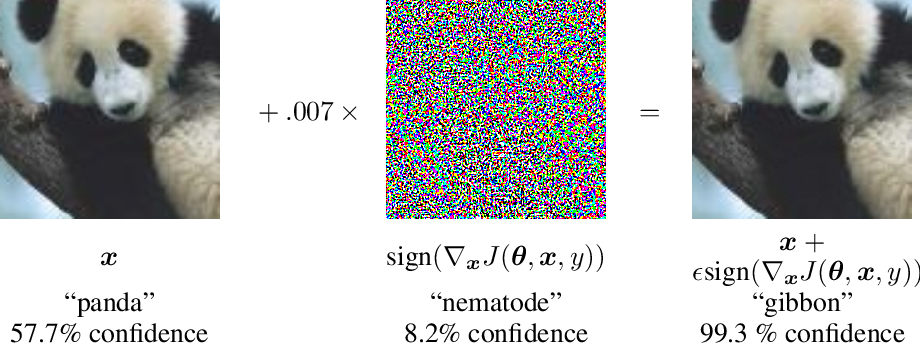
\includegraphics[width=0.5\textwidth]{images/goodfellow_panda.png}
    \caption{敵対的サンプルの例:パンダの敵対的サンプル画像によってテナガザルと誤分類する}
    \label{fig:adversarial_example}
\end{figure}

このような画像データに対する敵対的サンプルの生成は行うことができる.しかし,表形式データに対する敵対的サンプルは,先ほどの手法を用いて生成することは難しい.その理由として,表形式データの特徴量は画像データと異なる性質を持つためである.画像データの場合,各ピクセルの値は0から255の範囲の連続値として扱うことができ,わずかな変化は人間の目では認識できないことが多い.一方で,表形式データの特徴量には,年齢や収入といった数値データだけでなく,性別や職業といったカテゴリカルデータも含まれる.また,各特徴量は独立した意味を持っており,それぞれの特徴量の変化は明確な意味の変化を伴う.例えば,先ほどのパンダの画像の場合,個々のピクセル値にわずかな変化を加えても,人間にとってはそれが「パンダの画像」であることに変わりはない.しかし,ローン申請データにおいて,年収を示す特徴量に対してわずかな変化を加えた場合,その変化は申請者の経済状況を直接的に変えてしまう可能性がある.さらに,職業などのカテゴリカルデータの場合,わずかな変化という概念自体が適用できない.このような表形式データの特性により,画像データに対する敵対的サンプル生成手法をそのまま適用することは適切ではない.そこで,表形式データの特性を考慮した新たな敵対的サンプル生成手法が必要となる.特に,各特徴量の重要度や,特徴量の種類(連続値かカテゴリカル値か)を考慮した手法が求められる.

